\documentclass[11pt,a4paper]{article}
\usepackage[margin=2.2cm]{geometry}
\usepackage[T1]{fontenc}
\usepackage{lmodern}
\usepackage{graphicx}
\usepackage{booktabs}
\usepackage{float}
\usepackage{caption}
\usepackage{amsmath}
\usepackage{xcolor}
\usepackage{tikz}
\usepackage{enumitem}
\usepackage[hidelinks]{hyperref}
\setlist{itemsep=2pt,topsep=4pt}
\captionsetup{font=small,labelfont=bf}
\graphicspath{{../figures/}}
\newcommand{\nskilleventwindows}{2,508}\newcommand{\brskilleventwindows}{12.3\%}
\newcommand{\nskilleventdays}{1,849}\newcommand{\brskilleventdays}{12.3\%}
\newcommand{\nskilleventwindowsalltrain}{2,508}\newcommand{\brskilleventwindowsalltrain}{12.3\%}
\newcommand{\nskilljjas}{81,556}\newcommand{\brskilljjas}{12.3\%}
\newcommand{\nskilljjaseventwin}{2,098}\newcommand{\brskilljjaseventwin}{13.1\%}
\newcommand{\unitsratio}{896}\newcommand{\unitscorr}{0.561}
\newcommand{\code}[1]{\texttt{\small #1}}

\title{Can raw AIFS rainfall forecasts anticipate electricity-supply disruption during Indian floods?\\[4pt]
\large Methods, results and limitations of a first complete analysis (ESMI 2014--2018)}
\author{Flood-analysis project, \code{/scratch/users/ag4680/flood\_analysis}}
\date{23 September 2026}

\begin{document}
\maketitle
\tableofcontents
\clearpage

%======================================================================
\section{Summary}
\textbf{Question.} How far ahead can raw ECMWF AIFS precipitation forecasts (lead times of 1--5 days)
identify days of elevated electricity outages at Prayas ESMI voltage monitors during Indian flood events?
And how much skill is lost relative to observed IMD rainfall, the ``perfect-rainfall'' benchmark?

\medskip\noindent\textbf{Main findings.}
\begin{enumerate}
\item \textbf{Rain and outages are linked, but only weakly.} Heavier rain significantly raises the odds of a
disruption day: odds ratio $\approx 1.3$ per $e$-fold increase in $(1+\text{rain})$, $p<10^{-4}$, with the same
result in a model with a random intercept per station (Table~\ref{tab:coef}). In genuinely out-of-sample tests
(leave one flood episode out), the skill is small: ROC-AUC $\approx 0.56$--$0.57$ on flood-event windows,
against 0.54 for climatology, and Brier skill score (BSS) $\approx 0.005$--$0.01$ (Table~\ref{tab:skill-ev}).
\item \textbf{Skill hardly declines from day 1 to day 5.} AIFS rainfall itself degrades with lead: at the
3$\times$3 level its correlation with IMD falls from 0.73 to 0.66 (Table~\ref{tab:rain}). But the
rain$\rightarrow$outage signal is so weak that outage skill stays flat (AUC 0.573 at day 1, 0.572 at day 5).
\item \textbf{Replacing observed rain with the forecast costs almost nothing during floods.} On event windows,
AIFS at every lead matches IMD within noise. Over all June--September (JJAS) days, IMD is modestly better
(AUC 0.529 against 0.514--0.511).
\item \textbf{Persistence wins at day 1; AIFS wins at days 2--5.} Yesterday's outage is the best single
predictor at lead 1, and adding AIFS rain improves it (AUC 0.591 $\rightarrow$ 0.615). From lead 2 onward,
the latest known outage (day $D-L$) carries no information, but AIFS keeps its small skill.
\item \textbf{Urban, peri-urban and rural stations do not differ beyond noise.} Rural stations look best on
flood-event windows, but the rural and peri-urban event samples are small and the intervals overlap
(Table~\ref{tab:area}).
\end{enumerate}
\noindent The confidence intervals are wide (only 9 independent flood episodes), and several BSS intervals
include zero. The results describe a \emph{weak, marginally significant} signal, not usable operational skill.

%======================================================================
\section{Study design}
The design follows \code{docs/TASK.md}:
\begin{itemize}
\item \textbf{Units of analysis.} Station-days at ESMI monitors, 2014--2018.
\item \textbf{Flood events.} Global Flood Database (GFD; Tellman et al.\ 2021) events that inundate land near
a station during its ESMI coverage. This rebuilds the event set of Verschuur \& Balakrishnan (2024), who did
not publish their list.
\item \textbf{Predictors.} Daily rainfall at each station from AIFS at leads 1--5 days and, as a benchmark,
from IMD gauge analyses.
\item \textbf{Outcome.} A binary ``disruption day'' (outage minutes above the station's 90th percentile).
\item \textbf{Models.} Logistic models with climatology, persistence and IMD baselines.
\item \textbf{Validation.} Leave-one-flood-episode-out cross-validation, so every score describes a flood the
model has never seen, plus a leave-one-year-out analysis over the whole monsoon.
\end{itemize}

%======================================================================
\section{Data}
\begin{table}[H]\centering\small
\caption{Data sources.}
\begin{tabular}{p{3.1cm}p{5.3cm}p{6.8cm}}\toprule
Dataset & Content & Notes \\ \midrule
Prayas ESMI voltage & Minute-wise voltage, 10 CSVs, 2014--2018, 529 locations (metadata) & Wide format (one row per location-hour). Five files were truncated downloads and were re-downloaded from Harvard Dataverse (doi:10.7910/DVN/CLLZZM); all now match Dataverse byte for byte. \\
ESMI location information & District, state, category, connection type, From/To dates & No coordinates; categories map to urban / peri-urban / rural. \\
IMD gridded rainfall & 0.25$^\circ$ daily gauge analysis (Pai et al.\ 2014), 2014--2018 & 24\,h totals ending 08:30 IST (03 UTC) on the labelled date. \\
ECMWF AIFS forecasts & 1,818 daily 00 UTC initialisations (8 missing), 6-hourly steps to 120\,h, global 0.25$^\circ$ & Read-only source (8.5\,TB). India precipitation subset: 2.8\,GB. \\
Global Flood Database & MODIS 250\,m flood footprints; 26 events in and around India, 2014--2018 & Bands: \code{flooded}, \code{duration}, \code{clear\_views}, \code{clear\_perc}, \code{jrc\_perm\_water}. \\
\bottomrule\end{tabular}
\end{table}

%======================================================================
\section{Methods}
\subsection{ESMI processing (\code{scripts/01\_esmi\_profile\_daily.py})}
The minute data were reshaped into daily, per-location totals:
\begin{itemize}
\item \textbf{Outage minute:} voltage $<130$\,V, following Verschuur \& Balakrishnan. Exact 0\,V could also be
a monitor fault, but the two cannot be told apart, so 0\,V counts as an outage (owner decision).
\item \textbf{Observed day:} $\ge 90\%$ of the 1,440 minutes recorded. Missing rows are treated as monitor
downtime, not as outages. On other days the outage metrics are set to missing.
\item \textbf{Stations kept:} Agriculture connections are dropped, because farm feeders are rostered
(owner decision). Stations labelled \code{[Offline]} are kept, using only data within their From--To dates.
\end{itemize}
The result is 517 stations and 311,778 station-days inside coverage, of which 85.3\% are observed.

\subsection{Station coordinates (\code{scripts/02\_geocode\_locations.py})}
ESMI publishes only locality names with district and state. Locations were geocoded with Nominatim, with a
GeoNames fallback, constrained to the district. Of 529 stations:
\begin{itemize}
\item 300 are placed at the locality itself;
\item 212 fall back to the city centroid;
\item 17 fall back to the district centroid.
\end{itemize}
Each station is mapped to its nearest IMD cell with data. For 11 coastal stations the nearest cell has no
data, so the nearest cell with data is used instead (Figure~\ref{fig:loc}).

\begin{figure}[H]\centering
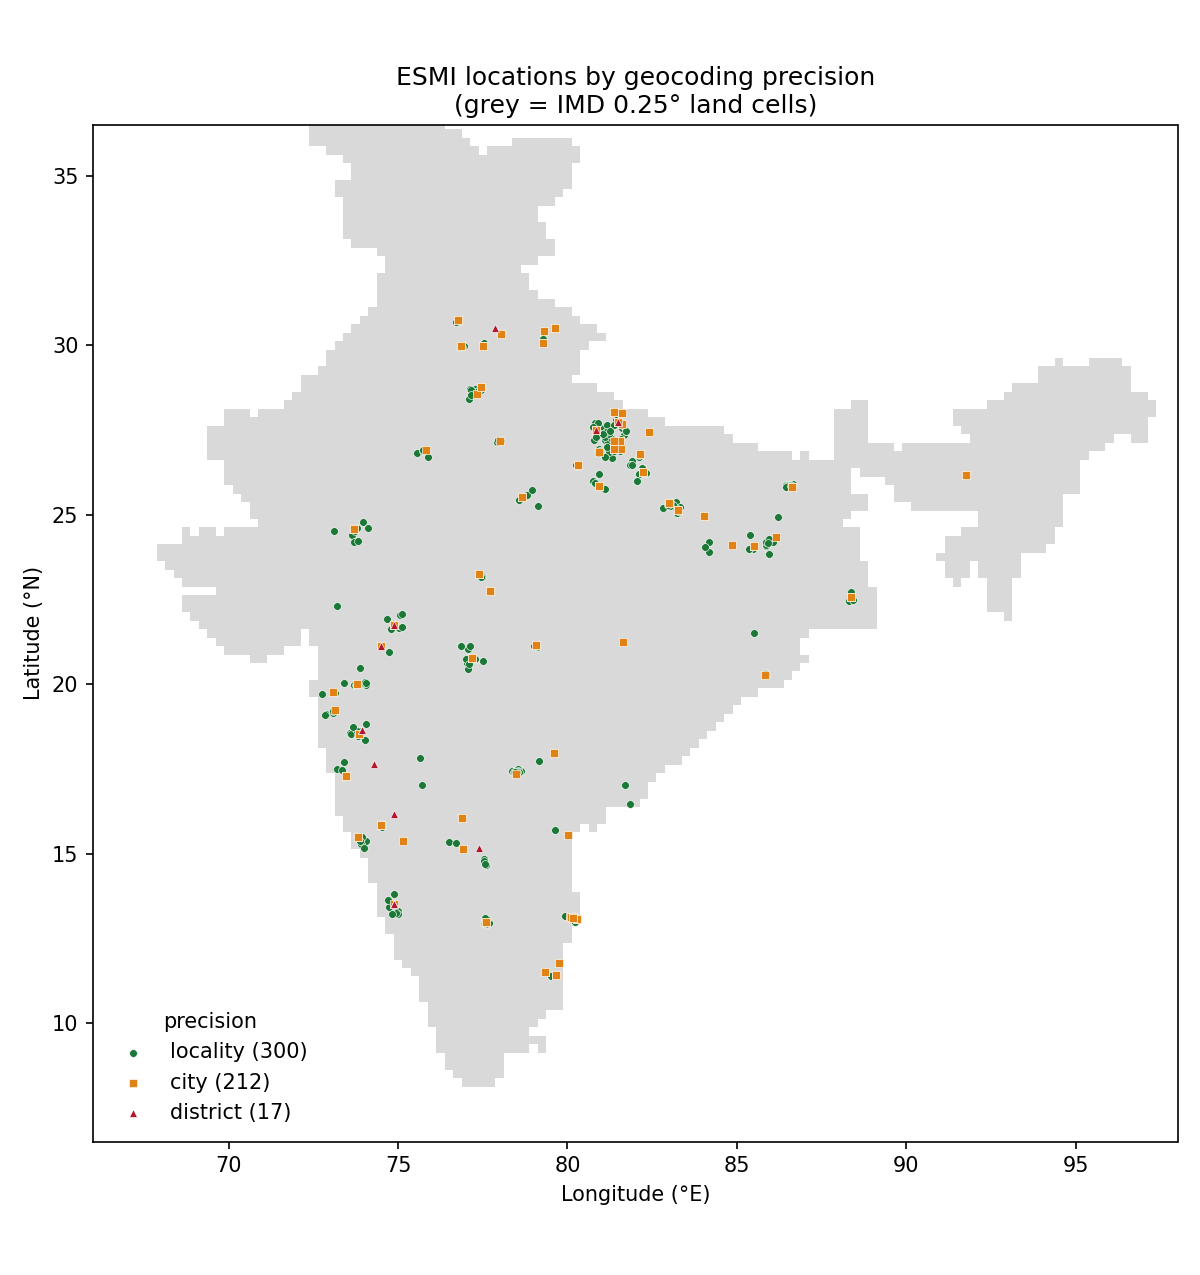
\includegraphics[width=0.62\textwidth]{02_locations_map.png}
\caption{Geocoded ESMI stations (\code{scripts/02}; review list in \code{outputs/02\_geocode\_review.csv}).}\label{fig:loc}
\end{figure}

\subsection{AIFS pre-processing and checks (\code{scripts/03}, \code{05})}
Only \code{total\_precipitation} over 5--40$^\circ$N, 65--100$^\circ$E was extracted (141$\times$141 points)
from every initialisation file, with NCO. The source files were never modified. Three checks were made:
\begin{itemize}
\item \textbf{Units: metres.} Over Indian land in July 2016, the median ratio of IMD daily rain (mm) to the
AIFS lead-1 daily sum is \unitsratio. A ratio of order 1,000 means metres; a ratio below 1,000 means AIFS is
about 12\% wetter than IMD over land ($1000/\unitsratio \approx 1.12$), consistent with the station-level wet bias in
Section~5.1. The mean spatial correlation for day 1 is \unitscorr.
\item \textbf{Step accumulation.} Values do not grow with lead time, so each step is a 6-hourly accumulation,
not a running total from initialisation.
\item \textbf{Initialisation and grid.} \code{time} $=0$ days since the init date and \code{leadtime}
$=6,12,\dots,120$\,h, so initialisation is at 00 UTC. The IMD grid points (6.5, 6.75, \dots$^\circ$N; 66.5,
\dots$^\circ$E) coincide exactly with AIFS points, so no regridding was needed.
\end{itemize}

\subsection{Time alignment (\code{scripts/06\_build\_panel.py})}
IMD and ESMI use Indian Standard Time (UTC+5:30); AIFS uses UTC.
\begin{itemize}
\item \textbf{IMD day $D$} runs from 03 UTC on $D-1$ to 03 UTC on $D$.
\item \textbf{AIFS lead $L$ for IMD day $D$} is the forecast initialised at 00 UTC on $D-L$, covering hours
$24(L-1)+3$ to $24L+3$ after initialisation. The two 6-hour steps straddling 03 UTC are split in half,
assuming uniform rain within a step:
\[
\text{AIFS}_L(D) = \tfrac12 s_{24L-18} + s_{24L-12} + s_{24L-6} + s_{24L} + \tfrac12 s_{24L+6},
\]
where $s_h$ is the step ending $h$ hours after initialisation.
\item \textbf{Lead 5 is approximate.} The forecast stops at 120\,h, so the step ending at 126\,h does not
exist. The 21 available hours are scaled by $24/21$.
\item \textbf{48-hour totals} add days $D-1$ and $D$ from the same forecast run, so they exist for leads 2--5
only.
\item \textbf{The ESMI day} (a calendar day in IST) runs from 18:30 UTC on $D-1$ to 18:30 UTC on $D$. It
overlaps the IMD day by 15.5\,h, and the IMD day leads it by 8.5\,h. IMD lags 0--2 are included to allow for
this offset.
\end{itemize}

\begin{figure}[H]\centering
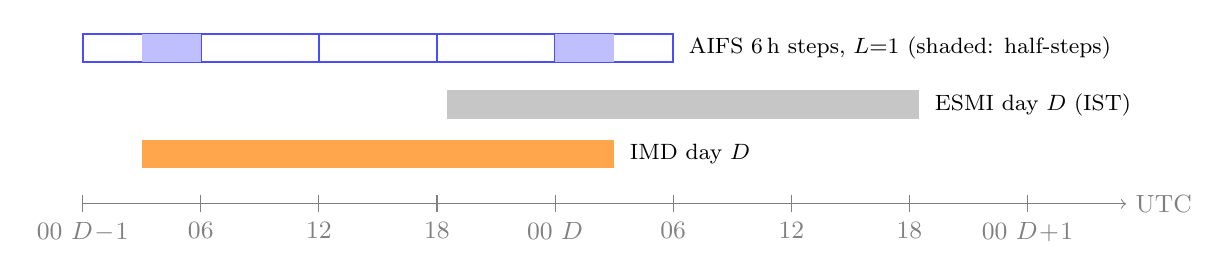
\begin{tikzpicture}[x=0.25cm,y=0.9cm,font=\small]
 \draw[->,gray] (0,0) -- (53,0) node[right]{UTC};
 \foreach \h/\l in {0/{00 $D\!-\!1$},6/06,12/12,18/18,24/{00 $D$},30/06,36/12,42/18,48/{00 $D\!+\!1$}}
   {\draw[gray] (\h,0.12)--(\h,-0.12) node[below]{\l};}
 \fill[orange!70] (3,0.5) rectangle (27,0.9); \node[right,font=\footnotesize] at (27.3,0.7){IMD day $D$};
 \fill[gray!45] (18.5,1.2) rectangle (42.5,1.6); \node[right,font=\footnotesize] at (42.8,1.4){ESMI day $D$ (IST)};
 \foreach \a in {0,6,12,18,24}{\draw[blue!70,thick] (\a,2.0) rectangle (\a+6,2.4);}
 \fill[blue!25] (3,2.0) rectangle (6,2.4); \fill[blue!25] (24,2.0) rectangle (27,2.4);
 \node[right,font=\footnotesize] at (30.3,2.2){AIFS 6\,h steps, $L{=}1$ (shaded: half-steps)};
\end{tikzpicture}
\caption{Time windows. For lead $L>1$ the AIFS steps are those of the forecast initialised $L$ days earlier.}
\end{figure}

\subsection{Spatial matching}
The centre cell is the nearest IMD cell with data; the same cell is used for AIFS. Three rain predictors were
computed: the centre cell, the 3$\times$3 mean ($\pm$0.25$^\circ$, about 25\,km) and the 3$\times$3 maximum.
Both 3$\times$3 versions use IMD-valid cells only, for both sources. The 3$\times$3 mean was fixed as the
headline predictor \emph{before} any results were seen; the other two are sensitivity checks.

\subsection{Flood-event reconstruction (\code{scripts/04\_match\_flood\_events.py})}
Verschuur \& Balakrishnan report 15 GFD events overlapping ESMI stations but did not publish the list, and
the authors declined to share it (they described the data quality as poor). The events were therefore
rebuilt from the 26 GFD footprints in and around India (Table~\ref{tab:events}):
\begin{enumerate}
\item \textbf{Flooded pixel:} GFD \code{flooded} $=1$ and not JRC permanent water.
\item \textbf{River-channel mask.} A first pass showed that \code{flooded} includes seasonally wet river
channels that JRC does not count as permanent. For example, the 11 Guwahati stations, 1--2\,km from the
Brahmaputra, ``matched'' 6 unrelated events, including one in March. Every footprint was therefore resampled
(nearest neighbour) onto a common 250\,m grid around each station, and pixels flooded in $\ge 3$ of the 26
events were masked as recurrent river water (owner decision).
\item \textbf{Affected station:} $\ge 1$\,km$^2$ of masked flooding within 20\,km. The paper's plain rule
(any flooded pixel within 20\,km) is kept as a sensitivity column.
\item \textbf{Event window:} GFD start $-3$ days to GFD end $+3$ days.
\item \textbf{Completeness:} the whole window must lie inside the station's ESMI coverage, and every day must
be observed. This implements the rule ``skip the event if observations are missing''.
\item \textbf{Episodes:} events whose windows overlap in time are merged into one episode for
cross-validation (4378+4382 in 2016; 4507+4508 in 2017), because they share the same rain and the same
station-days.
\end{enumerate}
The result is 11 events in 9 episodes, with 124 station-events at 84 stations. The plain rule would give 12
events and 226 station-events. Of the kept stations, 40 are placed at a city centroid, not the locality
itself.

\begin{table}[H]\centering
\caption{All 26 GFD footprints considered. ``Affected'': stations with $\ge1$\,km$^2$ of masked flooding
within 20\,km. ``In cov.'': of those, stations whose ESMI coverage overlaps the event. ``Kept'': the window is
fully covered and completely observed. ``Kept (raw)'': the same, under the plain 20\,km rule.}\label{tab:events}
\resizebox{\textwidth}{!}{\begin{tabular}{rllllrrrrl}\toprule ID & Country & Began & Ended & Cause & Affected & In cov. & Kept & Kept (raw) & Used \\ \midrule
4215 & Sri Lanka & 2014-12-20 & 2015-01-01 & Monsoonal Rain & 0 & 0 & 0 & 0 &  \\
4239 & India & 2015-03-20 & 2015-03-31 & Heavy Rain & 0 & 0 & 0 & 0 &  \\
4251 & India & 2015-05-17 & 2015-05-21 & Torrential Rain & 28 & 2 & 1 & 1 & yes \\
4259 & India & 2015-06-02 & 2015-06-29 & Monsoonal Rain & 11 & 0 & 0 & 0 &  \\
4265 & India & 2015-06-24 & 2015-06-29 & Monsoonal Rain & 0 & 0 & 0 & 0 &  \\
4272 & Pakistan & 2015-07-15 & 2015-08-19 & Monsoonal Rain & 0 & 0 & 0 & 0 &  \\
4282 & India & 2015-07-15 & 2015-08-19 & Monsoonal Rain and Tropical Storm  & 98 & 5 & 2 & 7 & yes \\
4283 & Myanmar & 2015-07-15 & 2015-08-19 & Monsoonal Rain & 0 & 0 & 0 & 0 &  \\
4288 & India & 2015-08-13 & 2015-09-11 & Monsoonal Rain & 11 & 0 & 0 & 0 &  \\
4309 & India & 2015-11-10 & 2015-12-04 & Tropical Storm Rovan & 44 & 15 & 5 & 8 & yes \\
4339 & Pakistan & 2016-03-12 & 2016-04-13 & Heavy Rain & 0 & 0 & 0 & 0 &  \\
4355 & India & 2016-04-20 & 2016-05-01 & Heavy Rain & 0 & 0 & 0 & 0 &  \\
4365 & Myanmar & 2016-06-01 & 2016-08-16 & Monsoonal Rain & 0 & 0 & 0 & 0 &  \\
4378 & India & 2016-07-07 & 2016-08-03 & Monsoonal Rain & 61 & 18 & 8 & 27 & yes \\
4382 & Bangladesh & 2016-07-25 & 2016-08-26 & Monsoonal Rain & 116 & 32 & 18 & 27 & yes \\
4459 & Bangladesh & 2017-03-30 & 2017-04-18 & Heavy Rain & 11 & 11 & 9 & 9 & yes \\
4483 & India & 2017-06-02 & 2017-07-03 & Monsoonal Rain & 11 & 11 & 10 & 10 & yes \\
4499 & India & 2017-07-27 & 2017-08-10 & Monsoonal Rain & 1 & 0 & 0 & 2 &  \\
4507 & India & 2017-08-10 & 2017-08-26 & Monsoonal Rain & 35 & 11 & 5 & 32 & yes \\
4508 & Bangladesh & 2017-08-10 & 2017-08-26 & Monsoonal Rain & 46 & 22 & 13 & 40 & yes \\
4632 & Myanmar & 2018-06-15 & 2018-06-20 & Monsoonal Rain & 0 & 0 & 0 & 0 &  \\
4640 & India & 2018-06-25 & 2018-07-11 & Monsoonal Rain & 0 & 0 & 0 & 0 &  \\
4645 & Pakistan & 2018-07-03 & 2018-07-11 & Monsoonal Rain & 0 & 0 & 0 & 0 &  \\
4666 & Myanmar & 2018-07-15 & 2018-08-10 & Monsoonal Rain & 0 & 0 & 0 & 0 &  \\
4665 & India & 2018-08-02 & 2018-08-10 & Monsoonal Rain & 11 & 6 & 5 & 5 & yes \\
4673 & India & 2018-09-01 & 2018-09-07 & Monsoonal Rain & 159 & 79 & 48 & 58 & yes \\
\bottomrule\end{tabular}}
\end{table}

\begin{figure}[H]\centering
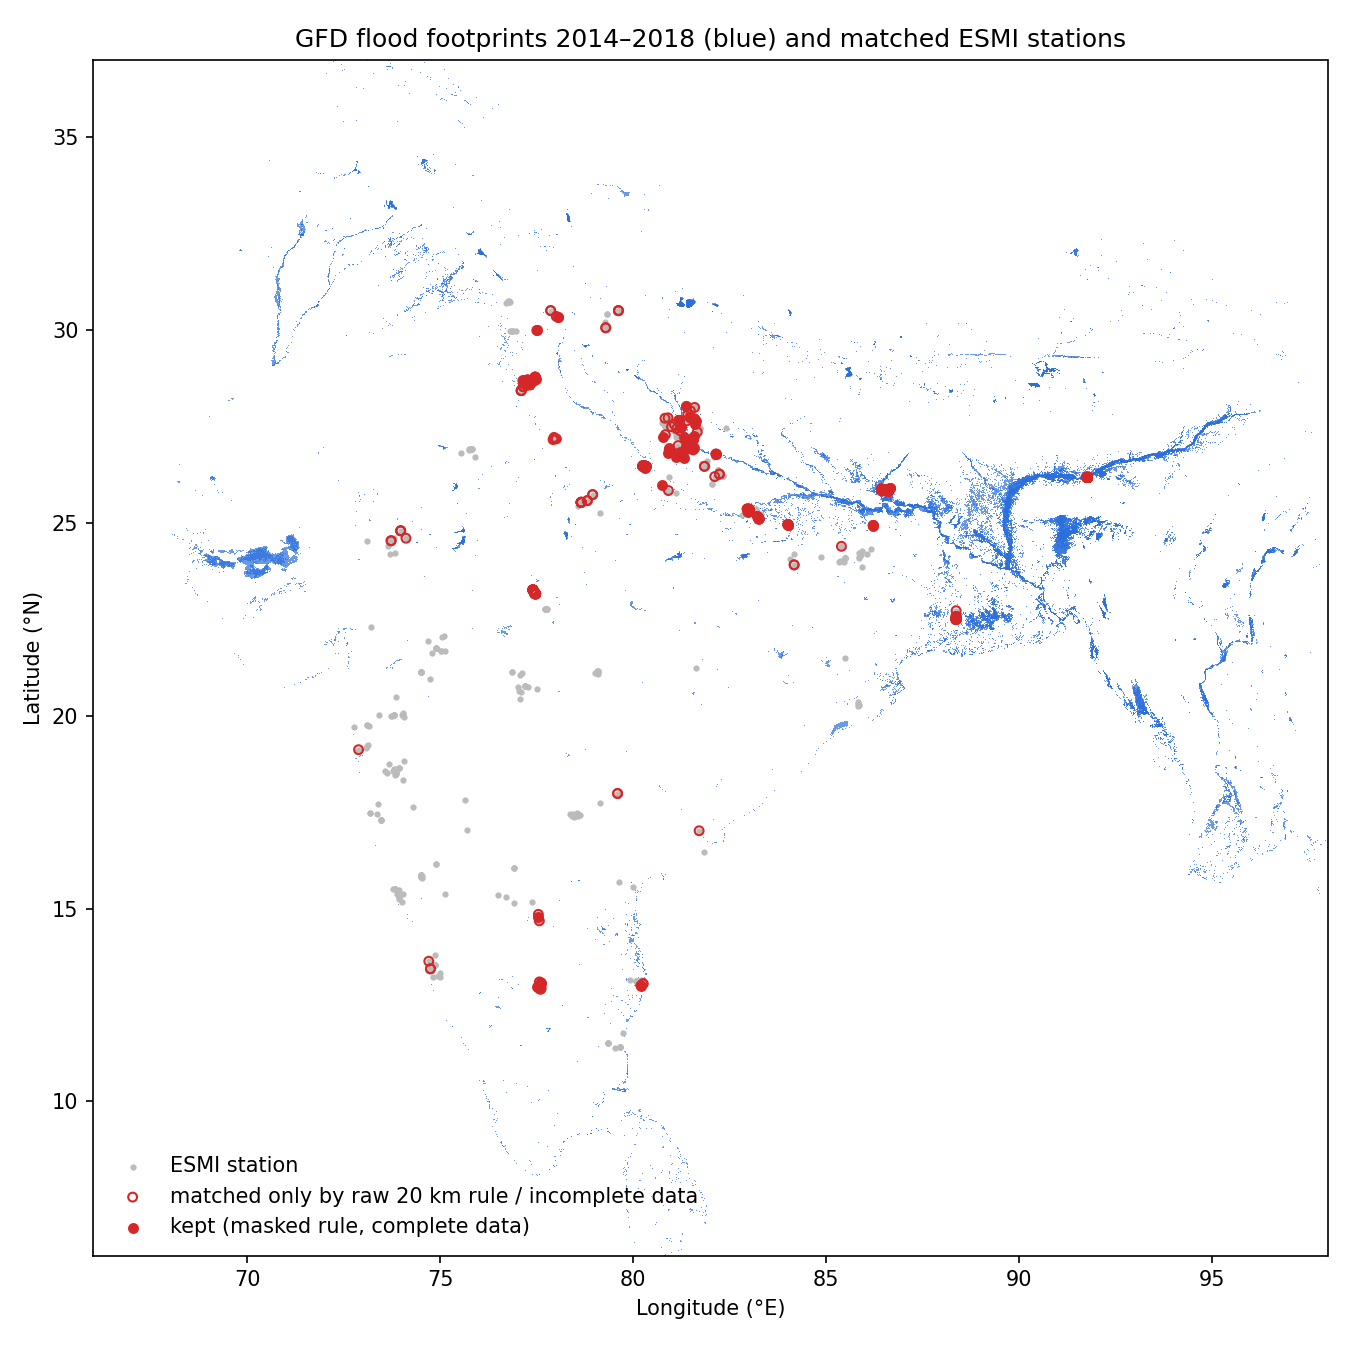
\includegraphics[width=0.72\textwidth]{04_flood_events_map.png}
\caption{GFD footprints, 2014--2018 (blue), and matched stations. Filled red: kept under the masked rule with
complete data. Open red: matched only by the plain rule, or with incomplete data.}\label{fig:floodmap}
\end{figure}

\subsection{Outcome definition}
\begin{itemize}
\item \textbf{Disruption day:} daily outage minutes above the station's 90th percentile. The percentile is
computed over observed days that are not near any flood (plain-rule windows excluded).
\item \textbf{Base rate:} 9.8\% of all station-days, 12.3\% in event windows and in JJAS. Floods and the
monsoon bring more outages, and 13 stations whose 90th percentile is 0 count any outage as a disruption.
\item \textbf{Secondary outcome:} excess minutes over the station's same-month, same-weekday median. This is
stored in the panel but not modelled in this pass.
\end{itemize}

\subsection{Models and baselines (\code{scripts/07\_model\_skill.py})}
Every model is a binomial GLM with climatology entered as an offset:
\[
\operatorname{logit}\Pr(\text{disrupt}_{s,D}) = \operatorname{logit} p^{\text{clim}}_{s,m(D)} + \beta_0 + \boldsymbol\beta^\top\mathbf x_{s,D}.
\]
Here $p^{\text{clim}}$ is the station $\times$ month disruption rate from the training fold, shrunk toward the
station rate (pseudo-count 20). Station, month and season are therefore controlled through the offset.
Predictors $\mathbf{x}$:
\begin{itemize}
\item \textbf{Climatology:} none (the offset alone).
\item \textbf{Persistence at lead $L$:} disruption on day $D-L$, the latest outage known when a lead-$L$
forecast is issued.
\item \textbf{AIFS 24\,h:} $\log(1+\text{rain})$ at lead $L$. \textbf{AIFS 48\,h:} the same for days $D-1$ and
$D$ from one forecast run ($L\ge2$).
\item \textbf{AIFS + persistence} at lead $L$.
\item \textbf{IMD benchmarks:} same day, 48\,h, and lags 0--2 (days $D$, $D-1$, $D-2$).
\end{itemize}
A random-intercept (per station) Bayesian mixed GLM, with month fixed effects fitted by variational Bayes,
serves as an in-sample check. IFS forecasts for 2014--2018 are not available, so they are not included.

\subsection{Cross-validation and scoring}
\begin{itemize}
\item \textbf{Event analysis: leave one flood episode out (9 folds).} The test set is the held-out episode's
event-window station-days. \emph{All dates} of that episode are removed from training for \emph{every}
station, to prevent leakage through spatially correlated days. Two training sets are used:
\begin{itemize}
\item \emph{event-only} (headline): the other episodes' event windows;
\item \emph{all days}: every other observed station-day.
\end{itemize}
\item \textbf{Monsoon analysis: leave one year out} over JJAS 2015--2018, trained on all days.
\item \textbf{Scores:} Brier score, BSS against climatology, ROC-AUC and reliability. All models are scored on
the same rows (every predictor available).
\item \textbf{Uncertainty:} 95\% intervals from a block bootstrap, resampling episodes for the event analysis
(1,000 draws) and stations for JJAS (200 draws).
\end{itemize}

%======================================================================
\section{Results}
\subsection{AIFS rainfall against IMD}
Over JJAS station-days, AIFS is about 0.8--1.0\,mm/day wetter than IMD at the centre cell and for the
3$\times$3 mean. Its 3$\times$3 maximum is about 6.5\,mm/day \emph{lower} than IMD's, because the gauge-based
IMD field has sharper local peaks. The correlation with IMD falls steadily with lead (Table~\ref{tab:rain},
Figure~\ref{fig:rain}). So the forecast degrades as expected: it is the outage link that is weak.

\begin{table}[H]\centering\small
\caption{AIFS against IMD daily rain at the stations, JJAS.}\label{tab:rain}
\begin{tabular}{rrrrrrr}\toprule & \multicolumn{3}{c}{Pearson $r$ with IMD} & \multicolumn{3}{c}{Bias AIFS$-$IMD (mm/day)} \\\cmidrule(lr){2-4}\cmidrule(lr){5-7} Lead (d) & centre & 3$\times$3 mean & 3$\times$3 max & centre & 3$\times$3 mean & 3$\times$3 max \\ \midrule
1 & 0.635 & 0.732 & 0.693 & +0.78 & +0.75 & -6.32 \\
2 & 0.626 & 0.721 & 0.682 & +1.01 & +0.99 & -6.26 \\
3 & 0.613 & 0.707 & 0.672 & +0.97 & +0.93 & -6.47 \\
4 & 0.596 & 0.688 & 0.655 & +0.83 & +0.79 & -6.67 \\
5 & 0.568 & 0.656 & 0.629 & +0.91 & +0.87 & -6.62 \\
\bottomrule\end{tabular}
\end{table}
\begin{figure}[H]\centering
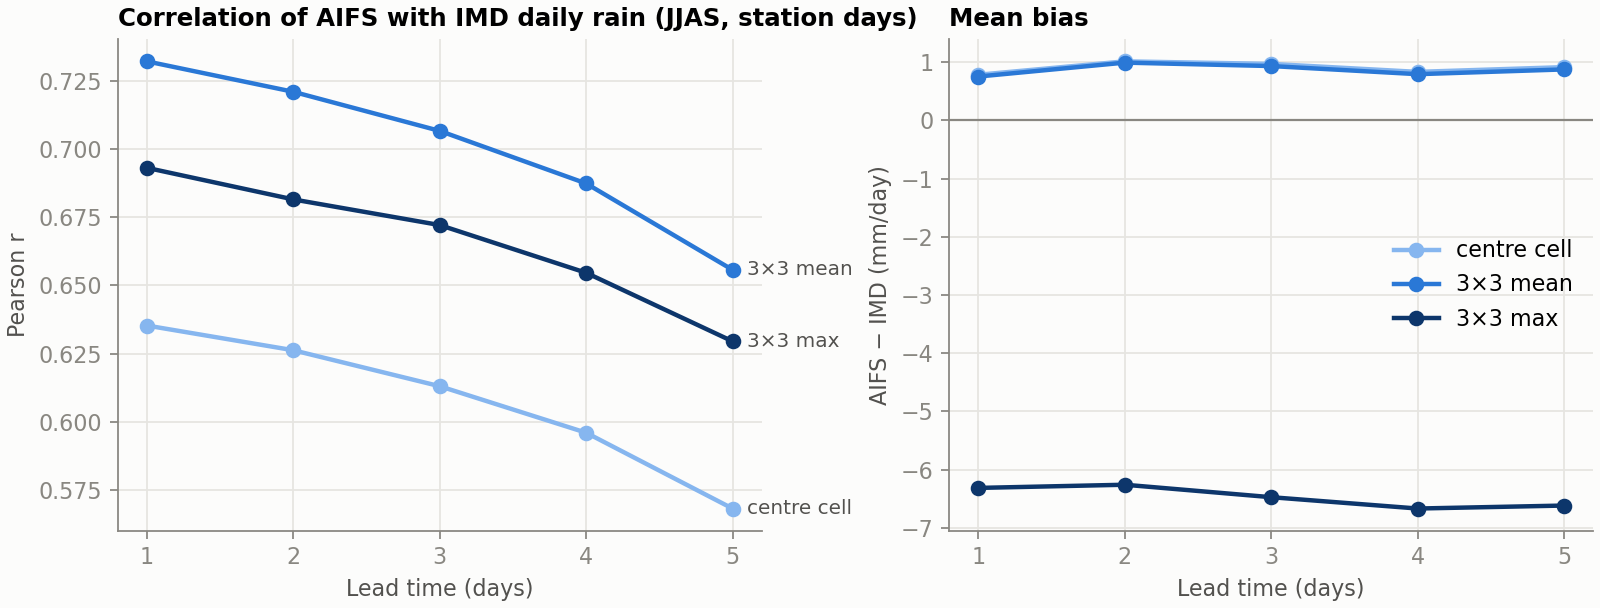
\includegraphics[width=\textwidth]{08_rain_vs_imd.png}
\caption{Correlation (left) and mean bias (right) of AIFS against IMD station rain, by lead and spatial
aggregation.}\label{fig:rain}
\end{figure}

\subsection{Event time series}
Figure~\ref{fig:ts} shows each episode. AIFS tracks the observed rain peaks at every lead, often with a wet
bias (episodes 7--9). Outage minutes, however, are dominated by station-specific baseline levels and noise.
For example, episode 4 begins at about 800\,min/day, before the flood peak. The two Kolkata stations in
episode 2 record no outages at all (CESC supply is very reliable).

\begin{figure}[H]\centering
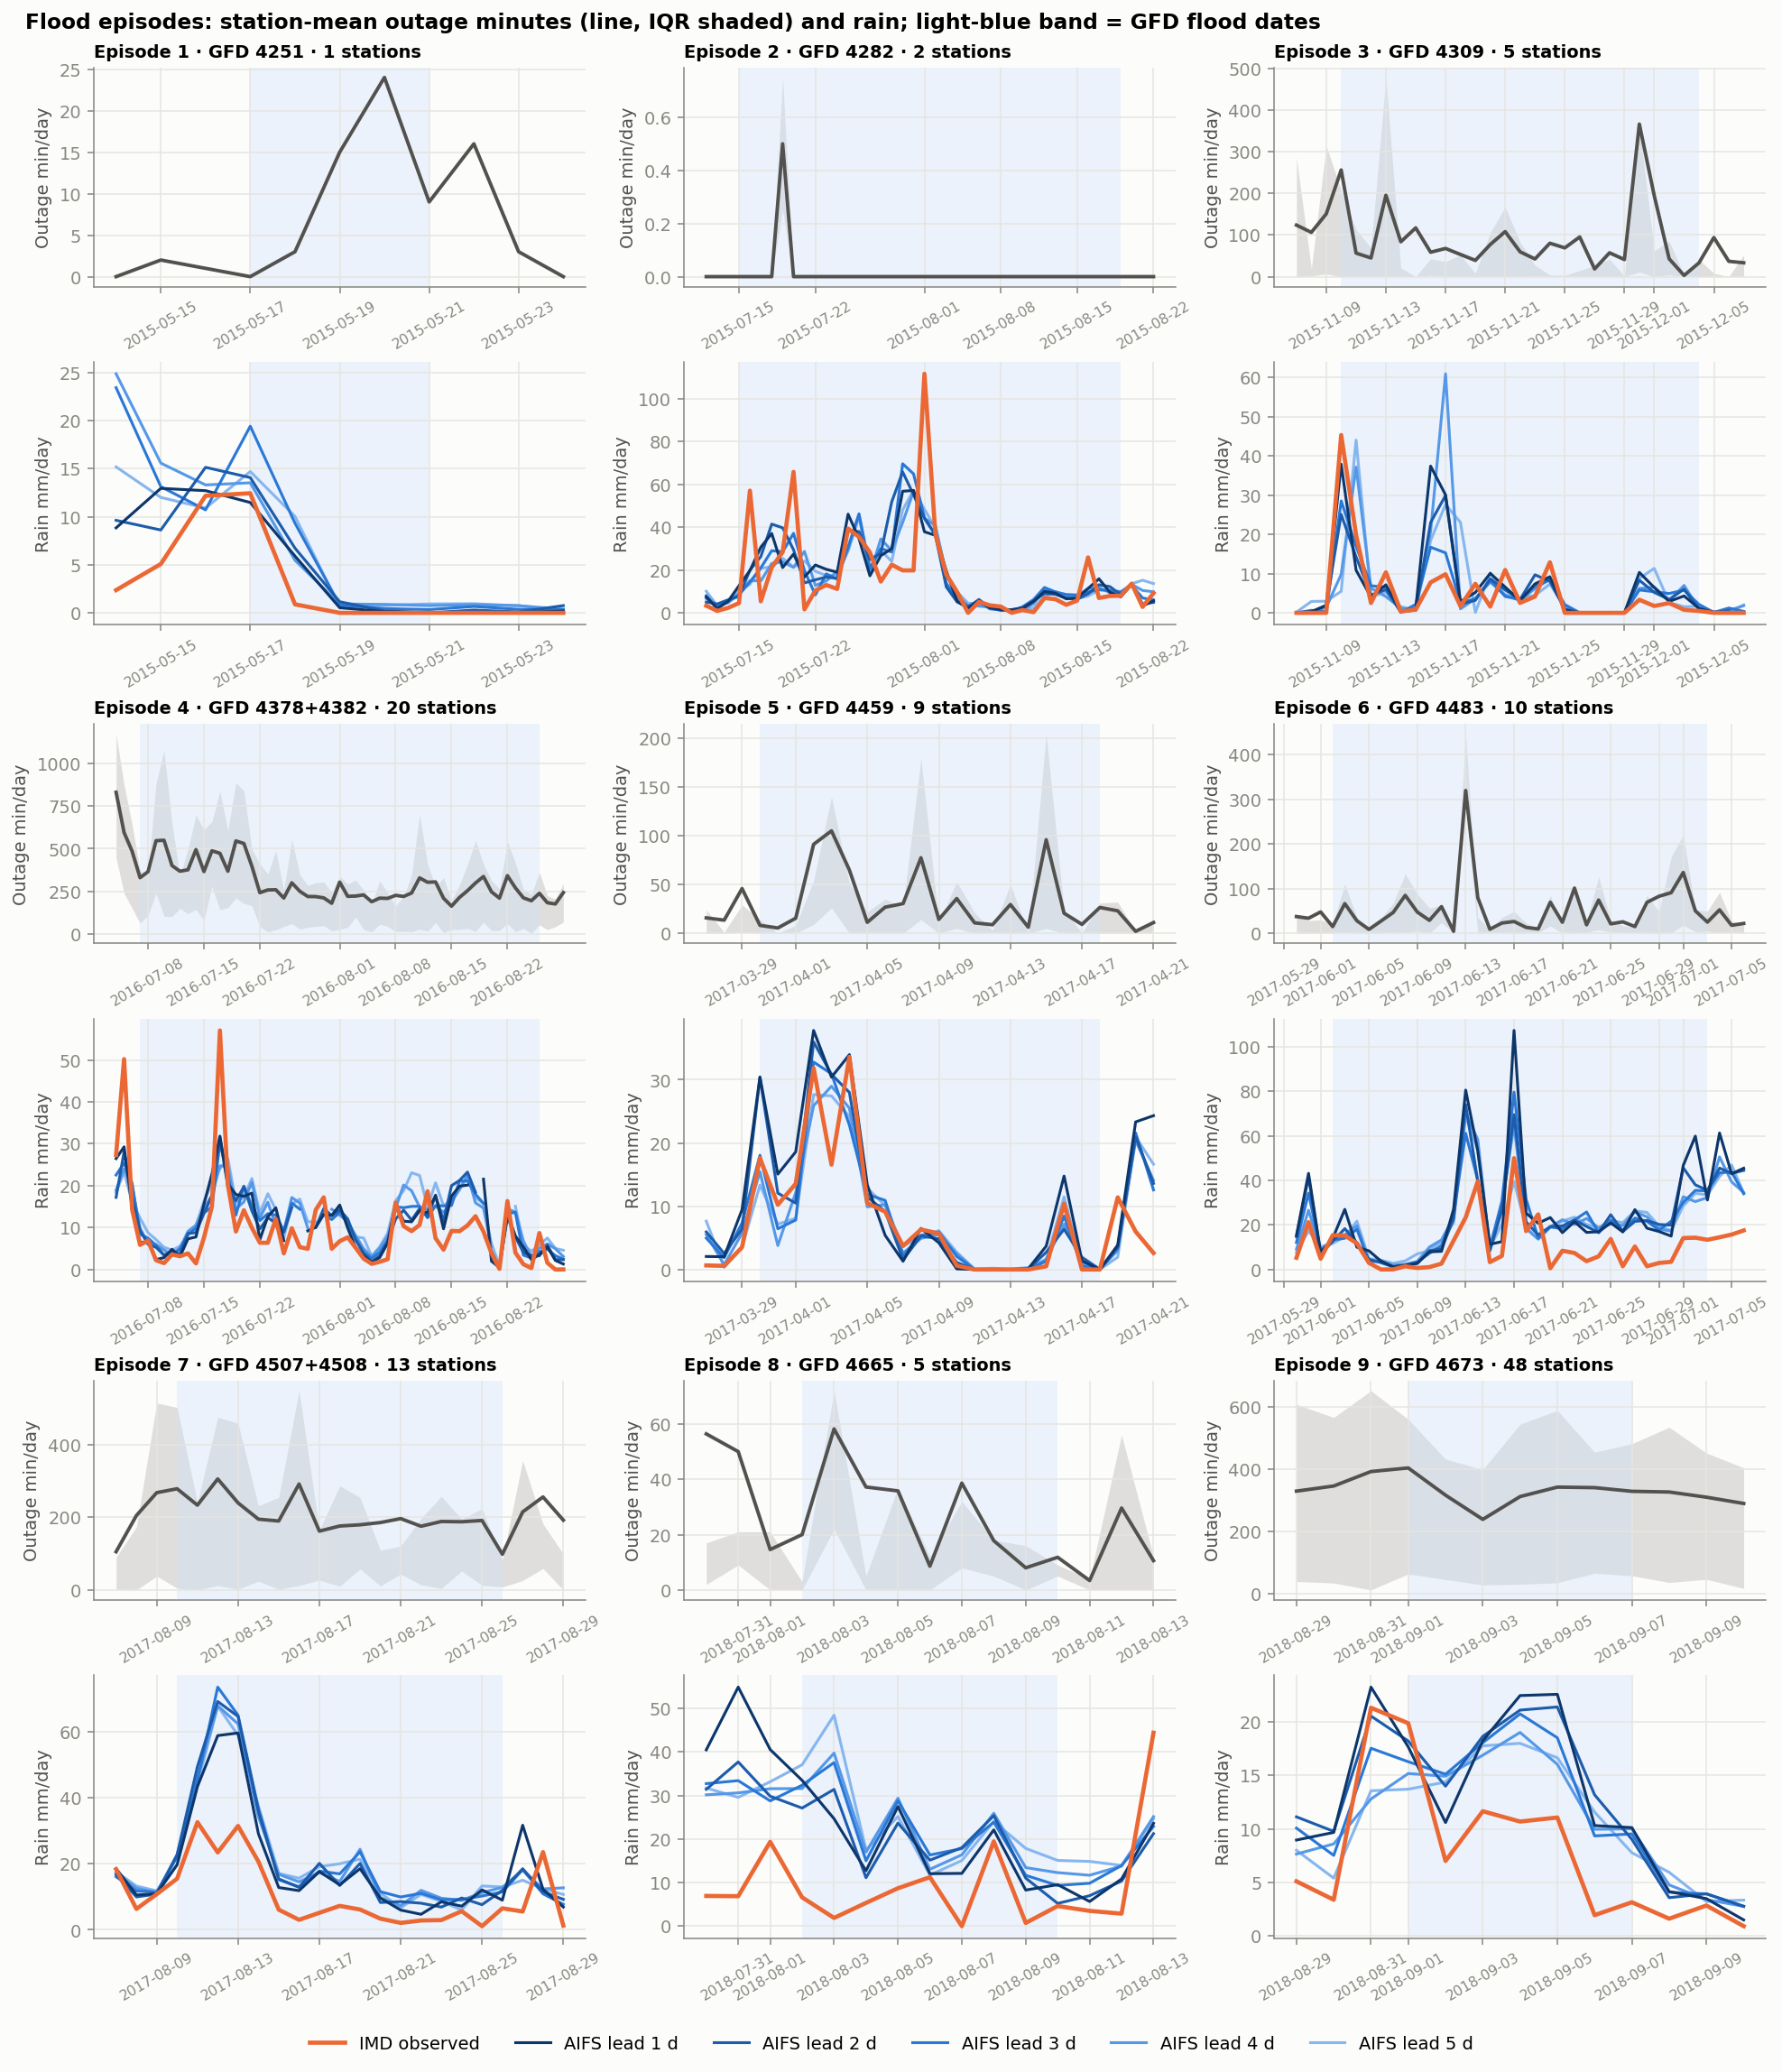
\includegraphics[width=\textwidth]{08_event_timeseries.png}
\caption{Per flood episode: station-mean outage minutes (line; interquartile range shaded) and station-mean
rain from IMD (orange) and AIFS at leads 1--5 (dark to light blue). Light-blue band: GFD flood dates.}\label{fig:ts}
\end{figure}

\subsection{Rain--outage association}
\begin{table}[H]\centering\small
\caption{In-sample coefficient on $\log(1+\text{rain})$ over event-window station-days ($n=2{,}508$). OR:
odds ratio per unit of $\log(1+\text{rain})$.}\label{tab:coef}
\begin{tabular}{lrrrrrrr}\toprule & \multicolumn{4}{c}{GLM, climatology offset} & \multicolumn{3}{c}{Random intercept per station} \\ \cmidrule(lr){2-5}\cmidrule(lr){6-8}Predictor & $\beta$ & SE & $p$ & OR & $\beta$ & SD & station SD \\ \midrule
IMD, day D & 0.239 & 0.056 & $<$0.001 & 1.27 & 0.215 & 0.028 & 0.72 \\
AIFS 24 h, lead 1 & 0.299 & 0.067 & $<$0.001 & 1.35 & 0.301 & 0.023 & 0.71 \\
AIFS 24 h, lead 2 & 0.308 & 0.072 & $<$0.001 & 1.36 & 0.307 & 0.023 & 0.71 \\
AIFS 24 h, lead 3 & 0.315 & 0.075 & $<$0.001 & 1.37 & 0.308 & 0.023 & 0.71 \\
AIFS 24 h, lead 4 & 0.313 & 0.077 & $<$0.001 & 1.37 & 0.299 & 0.023 & 0.71 \\
AIFS 24 h, lead 5 & 0.343 & 0.079 & $<$0.001 & 1.41 & 0.331 & 0.023 & 0.72 \\
\bottomrule\end{tabular}
\end{table}
\noindent The association is highly significant and consistent between the fixed and mixed models. The AIFS
coefficients are slightly larger than IMD's, so AIFS rain is at least as informative about outages as the
gauge analysis during these events. The station random-intercept SD ($\approx 0.7$ on the logit scale) shows
large differences between stations, which the climatology offset already absorbs.

\subsection{Cross-validated skill}
\begin{figure}[H]\centering
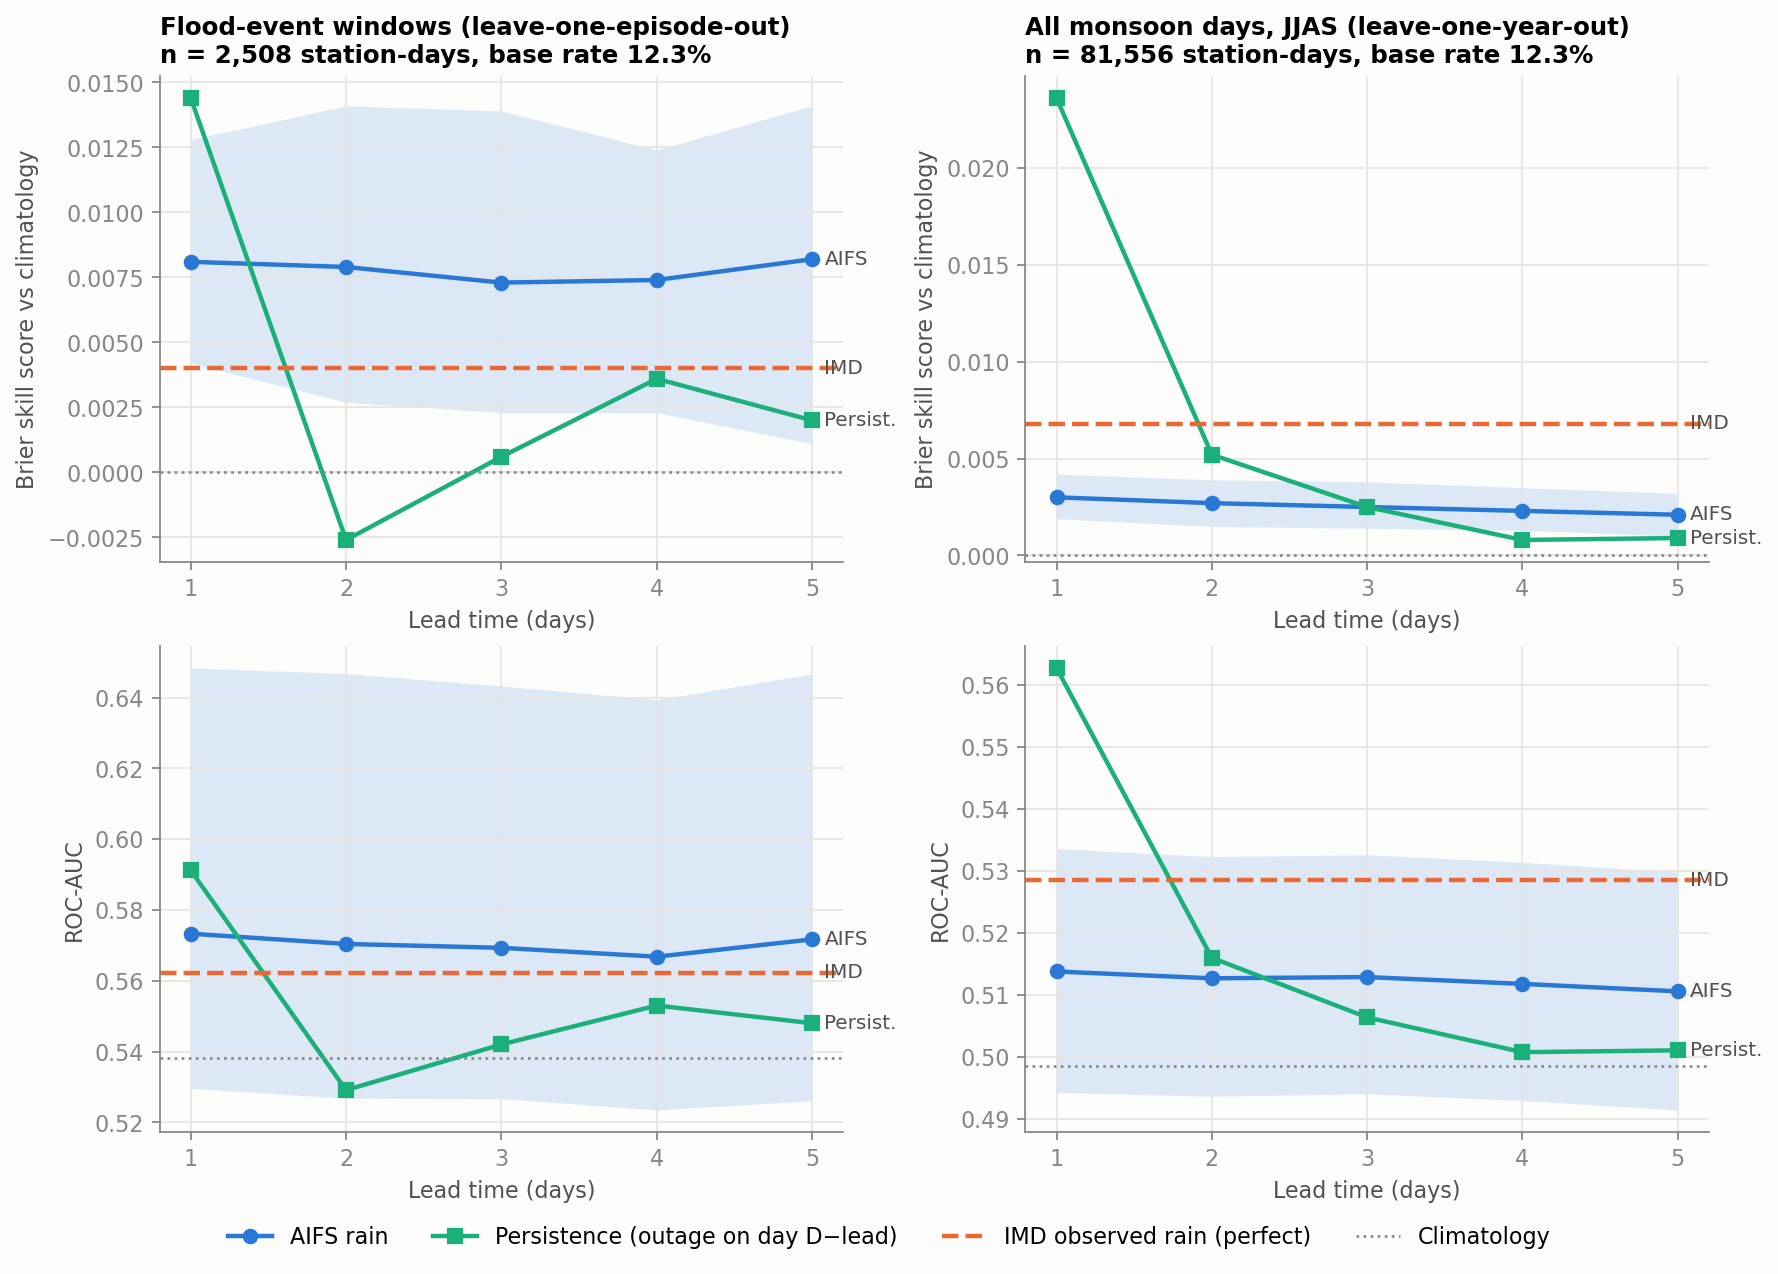
\includegraphics[width=\textwidth]{08_skill_vs_lead.png}
\caption{BSS (top) and ROC-AUC (bottom) against lead. Left: flood-event windows (leave one episode out,
event-only training). Right: all JJAS days (leave one year out). The blue band is the 95\% bootstrap interval
for AIFS.}\label{fig:skill}
\end{figure}

\begin{table}[H]\centering\small
\caption{Skill on flood-event windows, leave one episode out, event-only training
($n=\nskilleventwindows$, base rate \brskilleventwindows).}\label{tab:skill-ev}
\begin{tabular}{lrrcrc}\toprule
Model & Brier & BSS & 95\% CI & AUC & 95\% CI \\ \midrule
Climatology & 0.1090 & 0.000 & [0.000, 0.000] & 0.538 & [0.491, 0.612] \\
IMD, day D & 0.1085 & 0.004 & [-0.006, 0.011] & 0.562 & [0.515, 0.630] \\
IMD, 48 h & 0.1089 & 0.001 & [-0.008, 0.007] & 0.549 & [0.500, 0.623] \\
IMD, lags 0--2 & 0.1088 & 0.002 & [-0.011, 0.009] & 0.556 & [0.510, 0.621] \\
\midrule
Persistence, lead 1 & 0.1074 & 0.014 & [0.002, 0.024] & 0.591 & [0.539, 0.656] \\
Persistence, lead 2 & 0.1092 & -0.003 & [-0.011, 0.001] & 0.529 & [0.482, 0.604] \\
Persistence, lead 3 & 0.1089 & 0.001 & [-0.013, 0.007] & 0.542 & [0.491, 0.609] \\
Persistence, lead 5 & 0.1087 & 0.002 & [-0.007, 0.007] & 0.548 & [0.502, 0.619] \\
\midrule
AIFS 24 h, lead 1 & 0.1081 & 0.008 & [0.004, 0.013] & 0.573 & [0.530, 0.648] \\
AIFS 24 h, lead 2 & 0.1081 & 0.008 & [0.003, 0.014] & 0.570 & [0.527, 0.647] \\
AIFS 24 h, lead 3 & 0.1082 & 0.007 & [0.002, 0.014] & 0.569 & [0.527, 0.643] \\
AIFS 24 h, lead 4 & 0.1082 & 0.007 & [0.002, 0.012] & 0.567 & [0.523, 0.639] \\
AIFS 24 h, lead 5 & 0.1081 & 0.008 & [0.001, 0.014] & 0.572 & [0.526, 0.647] \\
\midrule
AIFS 48 h, lead 2 & 0.1086 & 0.003 & [-0.001, 0.007] & 0.555 & [0.509, 0.632] \\
AIFS 48 h, lead 5 & 0.1085 & 0.004 & [0.000, 0.008] & 0.559 & [0.513, 0.633] \\
\midrule
AIFS + persistence, lead 1 & 0.1068 & 0.020 & [0.006, 0.035] & 0.615 & [0.566, 0.683] \\
AIFS + persistence, lead 3 & 0.1082 & 0.007 & [0.002, 0.014] & 0.573 & [0.529, 0.643] \\
AIFS + persistence, lead 5 & 0.1079 & 0.009 & [0.004, 0.016] & 0.582 & [0.537, 0.653] \\
\bottomrule\end{tabular}
\end{table}

\begin{table}[H]\centering\small
\caption{Skill over all JJAS days, leave one year out ($n=\nskilljjas$, base rate \brskilljjas).}\label{tab:skill-jjas}
\begin{tabular}{lrrcrc}\toprule
Model & Brier & BSS & 95\% CI & AUC & 95\% CI \\ \midrule
Climatology & 0.1108 & 0.000 & [0.000, 0.000] & 0.498 & [0.480, 0.519] \\
IMD, day D & 0.1100 & 0.007 & [0.005, 0.008] & 0.528 & [0.510, 0.547] \\
IMD, 48 h & 0.1103 & 0.004 & [0.003, 0.005] & 0.518 & [0.499, 0.537] \\
IMD, lags 0--2 & 0.1098 & 0.009 & [0.007, 0.010] & 0.536 & [0.519, 0.553] \\
\midrule
Persistence, lead 1 & 0.1082 & 0.024 & [0.021, 0.027] & 0.563 & [0.547, 0.579] \\
Persistence, lead 2 & 0.1102 & 0.005 & [0.004, 0.006] & 0.516 & [0.499, 0.535] \\
Persistence, lead 3 & 0.1105 & 0.003 & [0.002, 0.003] & 0.506 & [0.489, 0.527] \\
Persistence, lead 5 & 0.1107 & 0.001 & [0.001, 0.001] & 0.501 & [0.484, 0.522] \\
\midrule
AIFS 24 h, lead 1 & 0.1104 & 0.003 & [0.002, 0.004] & 0.514 & [0.494, 0.534] \\
AIFS 24 h, lead 2 & 0.1105 & 0.003 & [0.002, 0.004] & 0.513 & [0.494, 0.532] \\
AIFS 24 h, lead 3 & 0.1105 & 0.003 & [0.001, 0.004] & 0.513 & [0.494, 0.533] \\
AIFS 24 h, lead 4 & 0.1105 & 0.002 & [0.001, 0.004] & 0.512 & [0.493, 0.531] \\
AIFS 24 h, lead 5 & 0.1105 & 0.002 & [0.001, 0.003] & 0.511 & [0.491, 0.530] \\
\midrule
AIFS 48 h, lead 2 & 0.1106 & 0.002 & [0.001, 0.002] & 0.507 & [0.488, 0.526] \\
AIFS 48 h, lead 5 & 0.1106 & 0.001 & [0.000, 0.002] & 0.506 & [0.487, 0.525] \\
\midrule
AIFS + persistence, lead 1 & 0.1080 & 0.025 & [0.022, 0.029] & 0.572 & [0.555, 0.587] \\
AIFS + persistence, lead 3 & 0.1102 & 0.005 & [0.004, 0.006] & 0.520 & [0.503, 0.540] \\
AIFS + persistence, lead 5 & 0.1104 & 0.003 & [0.002, 0.004] & 0.513 & [0.495, 0.532] \\
\bottomrule\end{tabular}
\end{table}

\paragraph{Reading the tables.}
\begin{itemize}
\item On event windows every rain model beats climatology, but only by 0.005--0.01 in BSS. AIFS is flat
across leads and on a par with IMD.
\item Over all JJAS days, climatology has AUC $\approx 0.5$ by construction, because the outcome is
station-relative, so every station has a similar base rate. There IMD beats AIFS, and AIFS declines slightly
with lead.
\item Persistence at lead 1 is the best single predictor in both samples, and adding AIFS rain improves on it.
At leads $\ge2$ persistence falls to the level of climatology.
\item The 48\,h totals and lags 0--2 add nothing over the single day.
\end{itemize}

\subsection{Reliability}
\begin{figure}[H]\centering
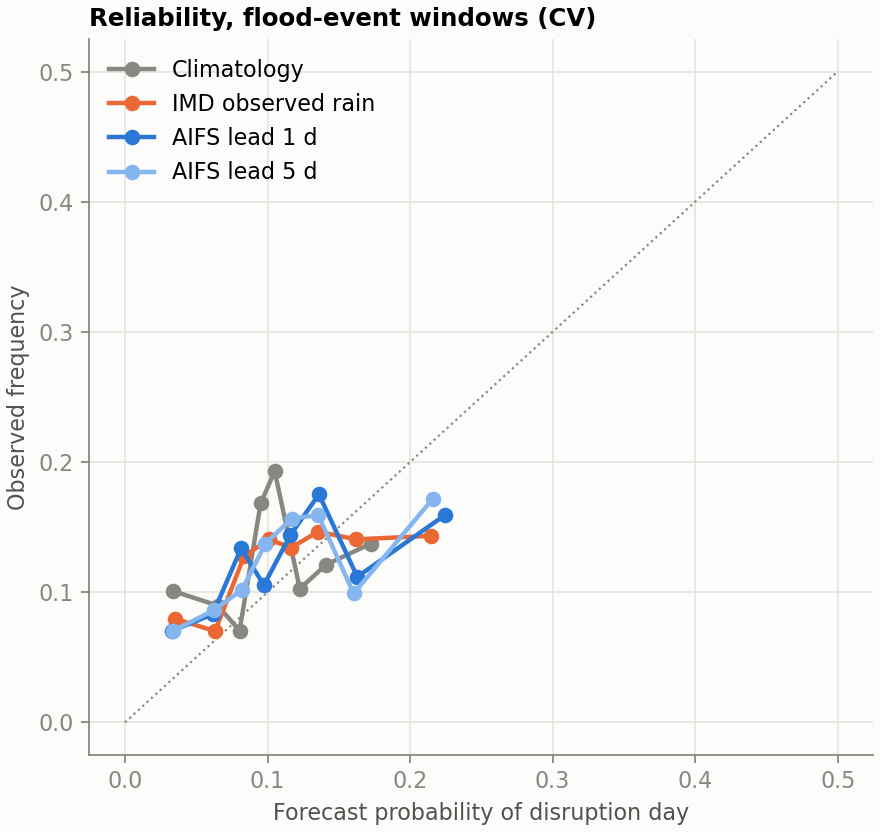
\includegraphics[width=0.5\textwidth]{08_reliability.png}
\caption{Reliability of the cross-validated event-window probabilities. The forecasts stay within
$\approx$0.03--0.22, so they are well calibrated but have little sharpness.}
\end{figure}

\subsection{Urban, peri-urban and rural}
\begin{table}[H]\centering\small
\caption{ROC-AUC by ESMI area type (3$\times$3 mean).}\label{tab:area}
\begin{tabular}{llrrrrrrr}\toprule Sample & Area & $n$ & Clim. & IMD & Pers. L1 & AIFS L1 & AIFS L3 & AIFS L5 \\ \midrule
Event windows & urban & 1,833 & 0.550 & 0.552 & 0.599 & 0.572 & 0.570 & 0.571 \\
Event windows & peri-urban & 104 & 0.540 & 0.594 & 0.530 & 0.561 & 0.531 & 0.528 \\
Event windows & rural & 571 & 0.494 & 0.590 & 0.572 & 0.587 & 0.579 & 0.588 \\
\midrule
JJAS all days & urban & 48,740 & 0.500 & 0.521 & 0.555 & 0.509 & 0.508 & 0.506 \\
JJAS all days & peri-urban & 10,990 & 0.507 & 0.544 & 0.578 & 0.528 & 0.527 & 0.525 \\
JJAS all days & rural & 21,826 & 0.488 & 0.537 & 0.571 & 0.517 & 0.516 & 0.512 \\
\bottomrule\end{tabular}
\end{table}
\begin{figure}[H]\centering
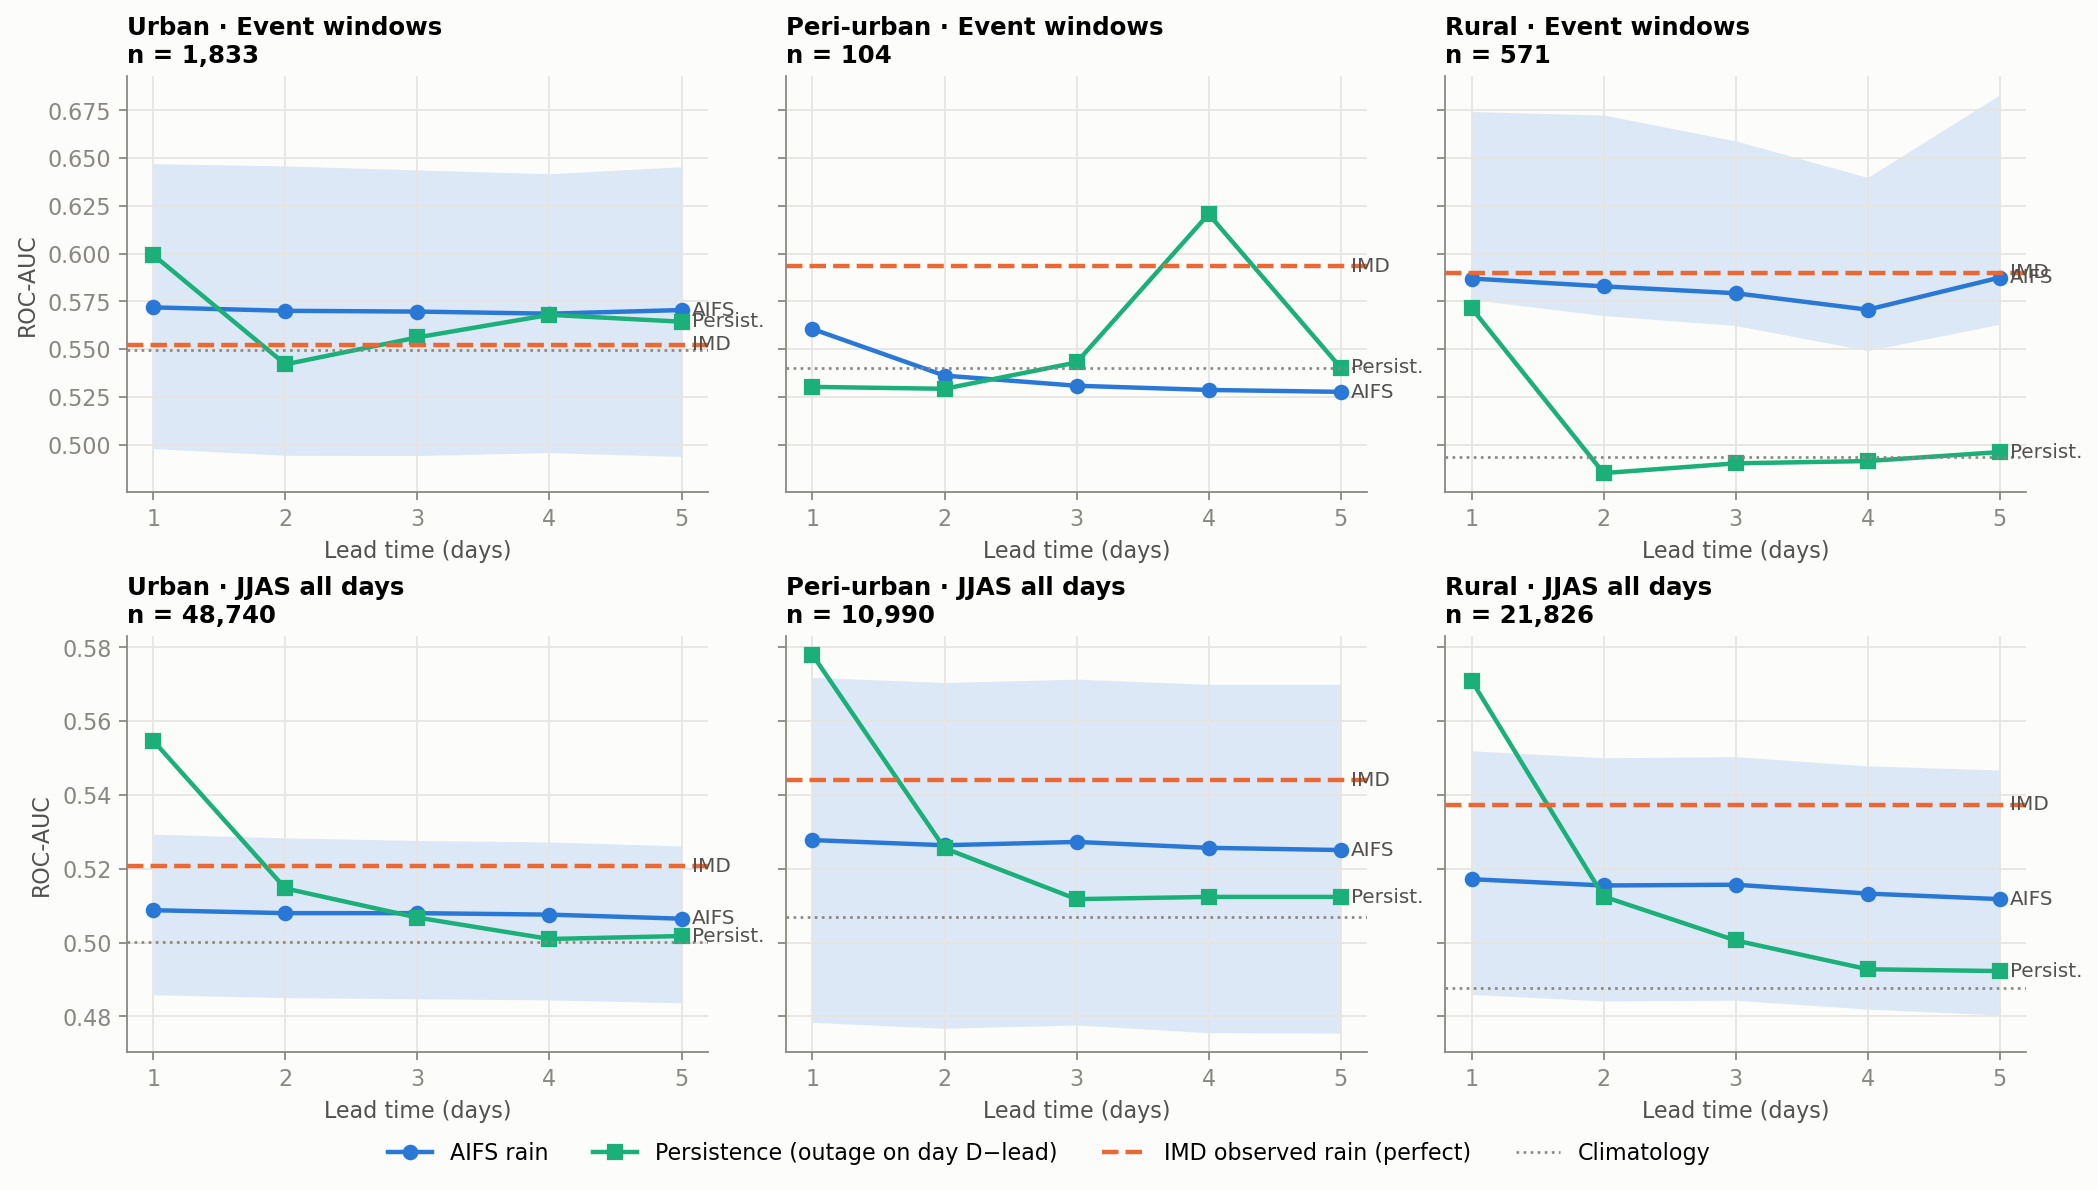
\includegraphics[width=\textwidth]{08_skill_by_area.png}
\caption{ROC-AUC against lead by area type. Top: event windows. Bottom: JJAS.}
\end{figure}
\noindent On flood-event windows, rural stations show the most rain skill (AIFS AUC $\approx$0.58--0.59, against 0.57 for
urban). Over all JJAS days, peri-urban and rural stations are similar and both slightly ahead of urban.
The peri-urban event sample is tiny ($n=104$) and all intervals overlap.

\subsection{Skill by episode}
\begin{table}[H]\centering
\caption{ROC-AUC by flood episode (event-only training). ``--'': no disruption days, so AUC is undefined.}\label{tab:ep}
\resizebox{\textwidth}{!}{\begin{tabular}{rllllrrrrrrrr}\toprule Ep. & GFD IDs & Country & Dates & Stn-events & $n$ & Base \% & Clim. & IMD & Pers. L1 & AIFS L1 & AIFS L5 \\ \midrule
1 & 4251 & India & 17 May 2015 -- 21 May 2015 & 1 & 11 & 0.0 & -- & -- & -- & -- & -- \\
2 & 4282 & India & 15 Jul 2015 -- 19 Aug 2015 & 2 & 84 & 1.2 & 0.380 & 0.651 & 0.373 & 0.566 & 0.651 \\
3 & 4309 & India & 10 Nov 2015 -- 04 Dec 2015 & 5 & 145 & 5.5 & 0.536 & 0.563 & 0.581 & 0.574 & 0.563 \\
4 & 4378+4382 & Bangladesh/India & 07 Jul 2016 -- 26 Aug 2016 & 26 & 664 & 12.3 & 0.588 & 0.610 & 0.640 & 0.614 & 0.606 \\
5 & 4459 & Bangladesh & 30 Mar 2017 -- 18 Apr 2017 & 9 & 234 & 9.8 & 0.481 & 0.631 & 0.573 & 0.633 & 0.611 \\
6 & 4483 & India & 02 Jun 2017 -- 03 Jul 2017 & 10 & 380 & 15.8 & 0.543 & 0.512 & 0.560 & 0.550 & 0.561 \\
7 & 4507+4508 & Bangladesh/India & 10 Aug 2017 -- 26 Aug 2017 & 18 & 299 & 17.4 & 0.479 & 0.495 & 0.501 & 0.503 & 0.494 \\
8 & 4665 & India & 02 Aug 2018 -- 10 Aug 2018 & 5 & 75 & 10.7 & 0.506 & 0.425 & 0.543 & 0.619 & 0.573 \\
9 & 4673 & India & 01 Sep 2018 -- 07 Sep 2018 & 48 & 616 & 12.0 & 0.483 & 0.533 & 0.577 & 0.516 & 0.502 \\
\bottomrule\end{tabular}}
\end{table}
\noindent Skill varies strongly between episodes. Episodes 1 and 2 have 0 and 1 disruption days, so their
AUCs are undefined or meaningless. Among the rest, skill is highest for the 2016 monsoon floods (episode 4,
AUC $\approx$0.61) and the April 2017 Assam/Bangladesh event (episode 5, $\approx$0.63). It is absent for the August 2017 floods (stations in Guwahati, Saharsa in Bihar, and
Uttar Pradesh) and the September 2018 event in northern India (mostly Uttar Pradesh), which contributes 48
of the 124 station-events.

\subsection{Sensitivity checks}
\begin{table}[H]\centering\small
\caption{ROC-AUC under different spatial aggregations.}
\begin{tabular}{llrrr}\toprule Sample & Model & Centre cell & 3$\times$3 mean & 3$\times$3 max \\ \midrule
Event windows & Climatology & 0.538 & 0.538 & 0.538 \\
Event windows & IMD, day D & 0.566 & 0.562 & 0.558 \\
Event windows & Persistence, lead 1 & 0.591 & 0.591 & 0.591 \\
Event windows & AIFS 24 h, lead 1 & 0.576 & 0.573 & 0.570 \\
Event windows & AIFS 24 h, lead 3 & 0.569 & 0.569 & 0.568 \\
Event windows & AIFS 24 h, lead 5 & 0.573 & 0.572 & 0.571 \\
Event windows & AIFS + persistence, lead 1 & 0.617 & 0.615 & 0.613 \\
\midrule
JJAS all days & Climatology & 0.498 & 0.498 & 0.498 \\
JJAS all days & IMD, day D & 0.528 & 0.528 & 0.525 \\
JJAS all days & Persistence, lead 1 & 0.563 & 0.563 & 0.563 \\
JJAS all days & AIFS 24 h, lead 1 & 0.514 & 0.514 & 0.512 \\
JJAS all days & AIFS 24 h, lead 3 & 0.513 & 0.513 & 0.511 \\
JJAS all days & AIFS 24 h, lead 5 & 0.511 & 0.511 & 0.509 \\
JJAS all days & AIFS + persistence, lead 1 & 0.572 & 0.572 & 0.570 \\
\bottomrule\end{tabular}
\end{table}
\begin{table}[H]\centering\small
\caption{Event days only (GFD start to end, no $\pm$3-day padding), event-only training ($n=\nskilleventdays$).}
\begin{tabular}{lrrcrc}\toprule
Model & Brier & BSS & 95\% CI & AUC & 95\% CI \\ \midrule
Climatology & 0.1089 & 0.000 & [0.000, 0.000] & 0.540 & [0.481, 0.617] \\
IMD, day D & 0.1087 & 0.003 & [-0.004, 0.007] & 0.553 & [0.506, 0.623] \\
IMD, 48 h & 0.1090 & -0.001 & [-0.007, 0.004] & 0.542 & [0.491, 0.612] \\
IMD, lags 0--2 & 0.1089 & 0.000 & [-0.005, 0.004] & 0.547 & [0.505, 0.617] \\
\midrule
Persistence, lead 1 & 0.1077 & 0.011 & [0.000, 0.022] & 0.585 & [0.542, 0.642] \\
Persistence, lead 2 & 0.1091 & -0.001 & [-0.007, 0.002] & 0.532 & [0.476, 0.605] \\
Persistence, lead 3 & 0.1091 & -0.001 & [-0.011, 0.005] & 0.539 & [0.473, 0.610] \\
Persistence, lead 5 & 0.1086 & 0.003 & [-0.005, 0.009] & 0.549 & [0.490, 0.620] \\
\midrule
AIFS 24 h, lead 1 & 0.1079 & 0.009 & [-0.000, 0.019] & 0.572 & [0.513, 0.650] \\
AIFS 24 h, lead 2 & 0.1079 & 0.009 & [-0.001, 0.021] & 0.572 & [0.512, 0.651] \\
AIFS 24 h, lead 3 & 0.1080 & 0.008 & [0.000, 0.018] & 0.569 & [0.511, 0.652] \\
AIFS 24 h, lead 4 & 0.1080 & 0.008 & [-0.001, 0.018] & 0.567 & [0.507, 0.648] \\
AIFS 24 h, lead 5 & 0.1079 & 0.010 & [-0.003, 0.021] & 0.571 & [0.507, 0.655] \\
\midrule
AIFS 48 h, lead 2 & 0.1087 & 0.003 & [-0.003, 0.007] & 0.552 & [0.496, 0.631] \\
AIFS 48 h, lead 5 & 0.1085 & 0.004 & [-0.003, 0.010] & 0.557 & [0.494, 0.639] \\
\midrule
AIFS + persistence, lead 1 & 0.1071 & 0.017 & [0.006, 0.032] & 0.608 & [0.563, 0.673] \\
AIFS + persistence, lead 3 & 0.1083 & 0.006 & [-0.001, 0.014] & 0.570 & [0.509, 0.646] \\
AIFS + persistence, lead 5 & 0.1077 & 0.012 & [-0.001, 0.023] & 0.579 & [0.514, 0.657] \\
\bottomrule\end{tabular}
\end{table}
\begin{table}[H]\centering\small
\caption{Event windows, models trained on all other days instead of event windows only ($n=\nskilleventwindowsalltrain$).}
\begin{tabular}{lrrcrc}\toprule
Model & Brier & BSS & 95\% CI & AUC & 95\% CI \\ \midrule
Climatology & 0.1090 & 0.000 & [0.000, 0.000] & 0.538 & [0.492, 0.615] \\
IMD, day D & 0.1082 & 0.007 & [-0.005, 0.016] & 0.568 & [0.519, 0.633] \\
IMD, 48 h & 0.1085 & 0.004 & [-0.007, 0.013] & 0.555 & [0.505, 0.626] \\
IMD, lags 0--2 & 0.1082 & 0.007 & [-0.004, 0.015] & 0.574 & [0.529, 0.633] \\
\midrule
Persistence, lead 1 & 0.1070 & 0.018 & [0.001, 0.033] & 0.604 & [0.552, 0.665] \\
Persistence, lead 2 & 0.1087 & 0.003 & [-0.007, 0.011] & 0.554 & [0.491, 0.623] \\
Persistence, lead 3 & 0.1085 & 0.004 & [-0.002, 0.009] & 0.553 & [0.509, 0.623] \\
Persistence, lead 5 & 0.1086 & 0.004 & [0.001, 0.006] & 0.551 & [0.502, 0.625] \\
\midrule
AIFS 24 h, lead 1 & 0.1083 & 0.006 & [-0.003, 0.013] & 0.565 & [0.517, 0.644] \\
AIFS 24 h, lead 2 & 0.1083 & 0.006 & [-0.003, 0.013] & 0.560 & [0.512, 0.641] \\
AIFS 24 h, lead 3 & 0.1083 & 0.006 & [-0.003, 0.013] & 0.559 & [0.512, 0.638] \\
AIFS 24 h, lead 4 & 0.1084 & 0.005 & [-0.003, 0.012] & 0.557 & [0.509, 0.636] \\
AIFS 24 h, lead 5 & 0.1083 & 0.006 & [-0.003, 0.012] & 0.557 & [0.509, 0.637] \\
\midrule
AIFS 48 h, lead 2 & 0.1085 & 0.004 & [-0.004, 0.010] & 0.551 & [0.502, 0.630] \\
AIFS 48 h, lead 5 & 0.1085 & 0.004 & [-0.004, 0.009] & 0.548 & [0.499, 0.629] \\
\midrule
AIFS + persistence, lead 1 & 0.1065 & 0.022 & [0.004, 0.041] & 0.620 & [0.567, 0.681] \\
AIFS + persistence, lead 3 & 0.1080 & 0.009 & [-0.004, 0.020] & 0.572 & [0.528, 0.641] \\
AIFS + persistence, lead 5 & 0.1080 & 0.009 & [-0.001, 0.016] & 0.569 & [0.517, 0.644] \\
\bottomrule\end{tabular}
\end{table}
\noindent The conclusions hold across all three checks. The spatial choice changes AUCs by less than 0.01: the centre cell is marginally highest and the
3$\times$3 maximum marginally lowest. Training on all days helps persistence slightly and leaves AIFS unchanged.

%======================================================================
\section{Caveats and limitations}
\begin{enumerate}
\item \textbf{ESMI data quality.} The authors of the reference study abandoned the flood--outage analysis
because of data quality. Monitor failures that record 0\,V are counted as outages, and monitor downtime
(missing rows) could correlate with floods. The strict completeness rule removes incomplete windows, but not
spurious zero readings.
\item \textbf{Weak outcome signal.} Outages are dominated by station-specific baselines and slow regime
changes (e.g.\ episode 4). A station-level 90th-percentile threshold absorbs the level but not these changes,
which dilutes the flood signal.
\item \textbf{Small number of independent events.} There are only 9 episodes, and one (Sept 2018, UP)
contributes 39\% of the station-events. The confidence intervals are wide and several include zero skill.
\item \textbf{Flood matching depends on choices.} The river-channel mask removes about 45\% of the plain-rule
station-events. The thresholds ($\ge3$ events, $\ge1$\,km$^2$, 20\,km) are judgement calls, and Guwahati still
matches three events on about 2\,km$^2$ of residual flooding. MODIS footprints also miss short-lived urban
flooding under cloud.
\item \textbf{Geocoding precision.} 40 of the 84 kept stations are placed at city centroids (errors of
roughly 5--10\,km). This is adequate for 20\,km buffers and the 0.25$^\circ$ rain grid, but it blurs
distance-based effects.
\item \textbf{Time alignment.} The IMD day and the ESMI day overlap by only 15.5\,h. The lead-5 total is
extrapolated from 21\,h, and the half-step split assumes uniform rain within each 6\,h step.
\item \textbf{Raw forecasts only.} AIFS is used without bias correction or ensembles. There is no IFS
comparison, and 8 initialisation dates are missing (their rows are dropped).
\item \textbf{Model simplicity.} A single log-rain term with a climatology offset. Nonlinear or threshold
effects (e.g.\ exceedance of a local rain percentile), outage counts, and interactions with grid
characteristics are not explored.
\item \textbf{Outcome not validated against reports.} There is no independent record of flood-related grid
shutdowns (e.g.\ utility press releases) against which to check the disruption days.
\end{enumerate}

%======================================================================
\section{Possible next steps}
\begin{enumerate}
\item Hand-fix the 40 kept city-centroid stations (\code{data/locations\_manual.csv}) and re-run scripts
04--10.
\item Use an outcome less sensitive to regime changes: excess minutes over a 30-day rolling median, and a
count or hurdle model for outage minutes.
\item Use extreme-rain predictors (exceedance of the station's 95th/99th rain percentile) instead of
$\log(1+\text{rain})$.
\item Sensitivity checks: the plain 20\,km rule, Domestic connections only, and 0\,V-only outages.
\item Add IFS or an AIFS ensemble if 2014--2018 hindcasts become available.
\end{enumerate}

%======================================================================
\appendix
\section{Pipeline and reproducibility}
\begin{table}[H]\centering\small
\begin{tabular}{p{5.4cm}p{10.2cm}}\toprule
Script & Output \\ \midrule
\code{00\_redownload\_esmi.sbatch} & Complete ESMI CSVs from Dataverse \\
\code{01\_esmi\_profile\_daily.py} & \code{data/esmi\_daily.csv.gz}, \code{esmi\_hourly.csv.gz}, file profile \\
\code{02\_geocode\_locations.py} & \code{data/locations.csv}, review list, station map \\
\code{03\_subset\_aifs\_india.sbatch} & \code{data/aifs\_india/*.nc} (precipitation, India) \\
\code{04\_match\_flood\_events.py} & \code{data/flood\_events.csv}, \code{flood\_event\_stations.csv}, flood map \\
\code{05\_check\_aifs\_units.py} & \code{logs/aifs\_units\_check.log} \\
\code{06\_build\_panel.py} & \code{data/panel\_daily.parquet} \\
\code{07\_model\_skill.py} & \code{outputs/07\_*.csv}; CV predictions \code{data/cv\_pred\_*.parquet} \\
\code{08\_figures.py} & \code{outputs/figures/08\_*.png} \\
\code{09\_make\_notebook.py} & \code{notebooks/01\_aifs\_outage\_skill.ipynb} \\
\code{10\_make\_report.py} & This report's tables; \code{10\_make\_report.sbatch} compiles the PDF \\
\bottomrule\end{tabular}
\end{table}
\noindent All heavy steps ran as Slurm jobs on Sherlock (logs in \code{logs/}) in the owner's
\code{jupyter\_notebook} environment. Every number in the tables is generated from the saved CSVs by
\code{scripts/10\_make\_report.py}.

\end{document}
